\chapter{Application} \label{chap:application}

\section{Objectives}

Considering the GLLAMM model developed in previous chapters, its application on a real data set had a four-fold purpose:

\begin{enumerate}
	%
	\item \textbf{Evaluate the performance of the parametrizations.} We assessed if changing the posterior sampling geometry benefited the performance of the MCMC method.
	%
	\item \textbf{Evaluate the retrodictive accuracy.} We wanted to assess how well the model retrodicted the data, and what was the evidence in favor of any of the proposed models.
	%
	\item \textbf{Assess the psychometric properties.} We had a special interest in determine how difficult the items were, and in what part of the abilities measurement range they were located.
	%
	\item \textbf{Test research hypothesis.} We were interested on testing hypothesis about the explanatory power a set of covariates had on the latent dimensions, and what were the implications of these, for the educational authority's policy decision making.
	%
\end{enumerate}

%%%%%%%%%%%%%%%%%%%%%%%%%%%%%%%%%%%%%%%%%%%%%%%%%%%%%%%%%%%%%%%%%%%%%%%

\section{Instrument}

The evaluation instrument was selected from the Peruvian public teaching career national assessment. The large standardized test took place during $2017$, an it allowed the winner to obtain an appointment, or temporal hiring, into the public teaching career of Peru. 

The instrument was composed of $90$ multiple-choice question, with four alternatives per item. The items were scored on a dichotomous scale, that is, only one of the four alternatives was the correct one. Moreover, the test was organized in three sub-tests designed to evaluate the reading comprehension, mathematical reasoning, and pedagogical knowledge of the applicants. Given the extension and differences between the sub-tests, we decided to focus on the reading comprehension portion, composed of the first $25$ items of the instrument. 

The reading comprehension sub-test was designed to evaluate the teacher's ability to reconstruct the meaning of different types of texts, presented in diverse formats. The sub-test had items designed to measure only one of the three hierarchically nested sub-dimensions of reading comprehension: literal, inferential, and reflective abilities. The literal ability items centered its focus on assessing the teacher's capability to locate explicit information on the texts. The inferential items assessed the teacher's ability to integrate the information in texts, with the goal of inferring its theme, purpose or implicit logic relationships. Lastly, the reflective items evaluated the teacher's abilities to critically reflect about the content and structure of texts.

Finally, besides being nested in dimensions, the items were bundled in groups of five, to a common text or passage, that provided the stimulus over which the individual was assessed, i.e. the items were testlets. 


%%%%%%%%%%%%%%%%%%%%%%%%%%%%%%%%%%%%%%%%%%%%%%%%%%%%%%%%%%%%%%%%%%%%%%%
%%%%%%%%%%%%%%%%%%%%%%%%%%%%%%%%%%%%%%%%%%%%%%%%%%%%%%%%%%%%%%%%%%%%%%%

\section{Data}

The data set was accessed through the proper legal requirement of open information to the Ministry of Education of Peru (MINEDU). The data was anonymized and transferred through digital mean to the researcher.

Finally, given the large amount of individuals exposed to the aforementioned evaluation (approximately $195,000$), a simple random sample of $2,000$ individuals was taken. 

%%%%%%%%%%%%%%%%%%%%%%%%%%%%%%%%%%%%%%%%%%%%%%%%%%%%%%%%%%%%%%%%%%%%%%%
%%%%%%%%%%%%%%%%%%%%%%%%%%%%%%%%%%%%%%%%%%%%%%%%%%%%%%%%%%%%%%%%%%%%%%%

\section{Hypothesis}

On it core, statistical models are neat association engines. Through their use, one is able to detect associations between variables, and estimate their effects. However, when a researcher find itself in the position of trying to determine what are the consequences of intervening on a variable, i.e. infer causes, statistical models are never sufficient. Information outside the data, related to the causal hypothesis between the variables, is always required \cite{McElreath_2020}. Nevertheless, since much of time the statistical endeavor has to do with produce understanding that leads to generalization and application; there must be a reasonable way to state our hypothesis, and to think formally about causal inference.

Luckily, as \citet{McElreath_2020}, \citet{Hernan_et_al_2020}, and several other authors indicate, Graphical Causal Models (GCM) can come to the rescue. The simplest and yet powerful GCM is the Directed Acyclic Graph (DAG). A DAG is a heuristic model that contains information that is not purely statistical, but unlike a detailed statistical model, the graph allow us to deduce which variable relationships can provide valid causal inferences. However, abide by the ``no-free lunch" rule, the causal inferences produced under a DAG are only valid if the assumed DAG is correct. On the latter, one would think the aforementioned caveat is an insurmountable critic of the tool, but one would forget that any statistical analysis hinges on assumption, and a DAG is just a tool to make assumptions more transparent. A full description of the GCM formal theory is beyond the scope of this work. However, if the reader is interested in the topic, he/she can refer to \citet{McElreath_2020} or  \citet{Hernan_et_al_2020} for introductory level descriptions, and beyond, about the use of GCM for the statistical endeavor.

So, for our current research interest, figures \ref{fig:FOLV_app} and \ref{fig:SOLV_app} show the DAGs of the application's first- and second-order latent variable model (FOLV and SOLV, respectively). The figures aim to reflect the hierarchies and hypothesized dimensional structure of the instrument, while also describing the assumed qualitative relationships among the structural covariates. 

A careful inspection of both figures reveal they are similar to the ones implemented in the previous chapter. Therefore, the definitions of the likelihoods, priors, and \textit{hyper-priors} will be similar in nomenclature and even in distributional assumptions, as the simulated counterparts (see appendix \ref{appC3:chapter5} to corroborate the statement). Nevertheless, the previous cannot be fully extended to the structural covariates, as one can notice the models have a different set of variables than their simulated counterparts. Consequently, in this section we proceed to define them and outline their assumed causal hypothesis.

It is important to emphasize, the hypothesis presented in this section, and the results presented in section \ref{sect:test_hypothesis}, will take a diagnostic perspective, that is, we will emphasize on what factors does the educational authorities will need to give priority, to ensure a fair and equitable development of teachers.
%
\begin{figure}[H]
	\centering
	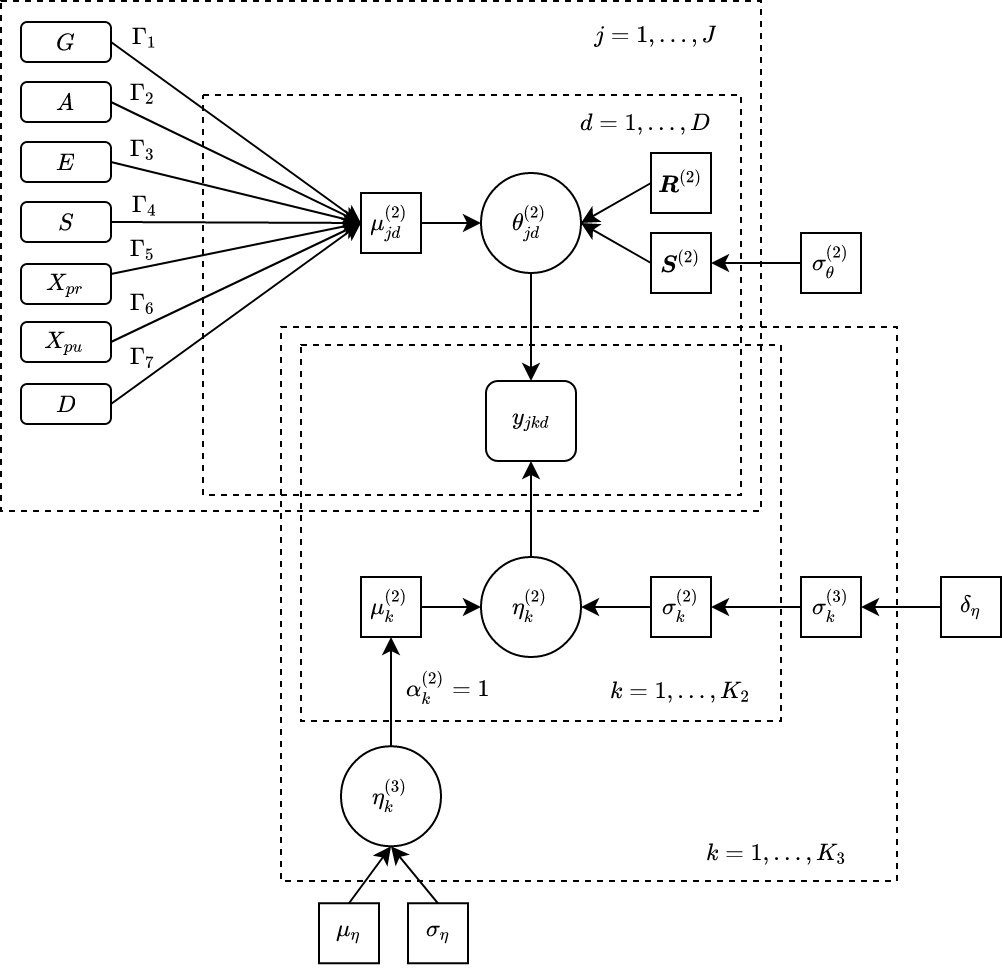
\includegraphics[width=0.8\linewidth]{app_FOLV_dag}
	%
	\caption[Directed Acyclic Graph (DAG). Application's first-order latent variable model (FOLV).]%
	{Directed Acyclig Graph (DAG). Application's first-order latent variable model (FOLV). Circles represent latent variables. Squares represent parameters or parameters for priors. Large squares represent nesting in specific units.}
	\label{fig:FOLV_app}
\end{figure}

First, we assumed the reading abilities and/or sub-dimensions were affected by age ($A$). In this particular case, age was used as a proxy for the applicant's style of teaching. As it is point out by the current National Basic Regular Educational Curriculum of Peru\footnote{National Basic Regular Educational Curriculum (2017). URL: \url{ http://www.minedu.gob.pe/curriculo/pdf/curriculo-nacional-2016-2.pdf} }, approximately forty years ago, an individual was considered literate if he/she had acquired the basic knowledge of reading, writing, and performing mathematics; while having a preliminary exposure to trades's dexterity and abilities. Much of this has been changing throughout the years, and although reading and writing abilities remained important, the criteria to determine if a person is literate, now goes beyond assessing if an individual knows the basic of how to read, write, or apply mathematics. Therefore, it is sensible to assume, age could inform us if a participant has a style of teaching based on the previous requirements of literacy (what we dubbed as the ``old" curricula). The idea is that older applicants, having developed most of their educational careers under the ``old" curricula, now being assessed under the new one, would register lower levels of reading comprehension. However, since the evolution from the ``old" to the new curricula is not a binary scenario, i.e. you either are in one or the other; but rather a continuous evolution, we reflect this idea by allowing age explain the abilities on a continuous manner, more specifically, a linear one. Off course, since age is associated with several other factors, e.g. cognitive development, we understand the previous hypothesis would not be the only one explaining the outcome. However, we believe that by measuring this effect, albeit proxy, educational authorities could be able to target in-training services to individuals with these characteristics.
%
\begin{figure}[H]
	\centering
	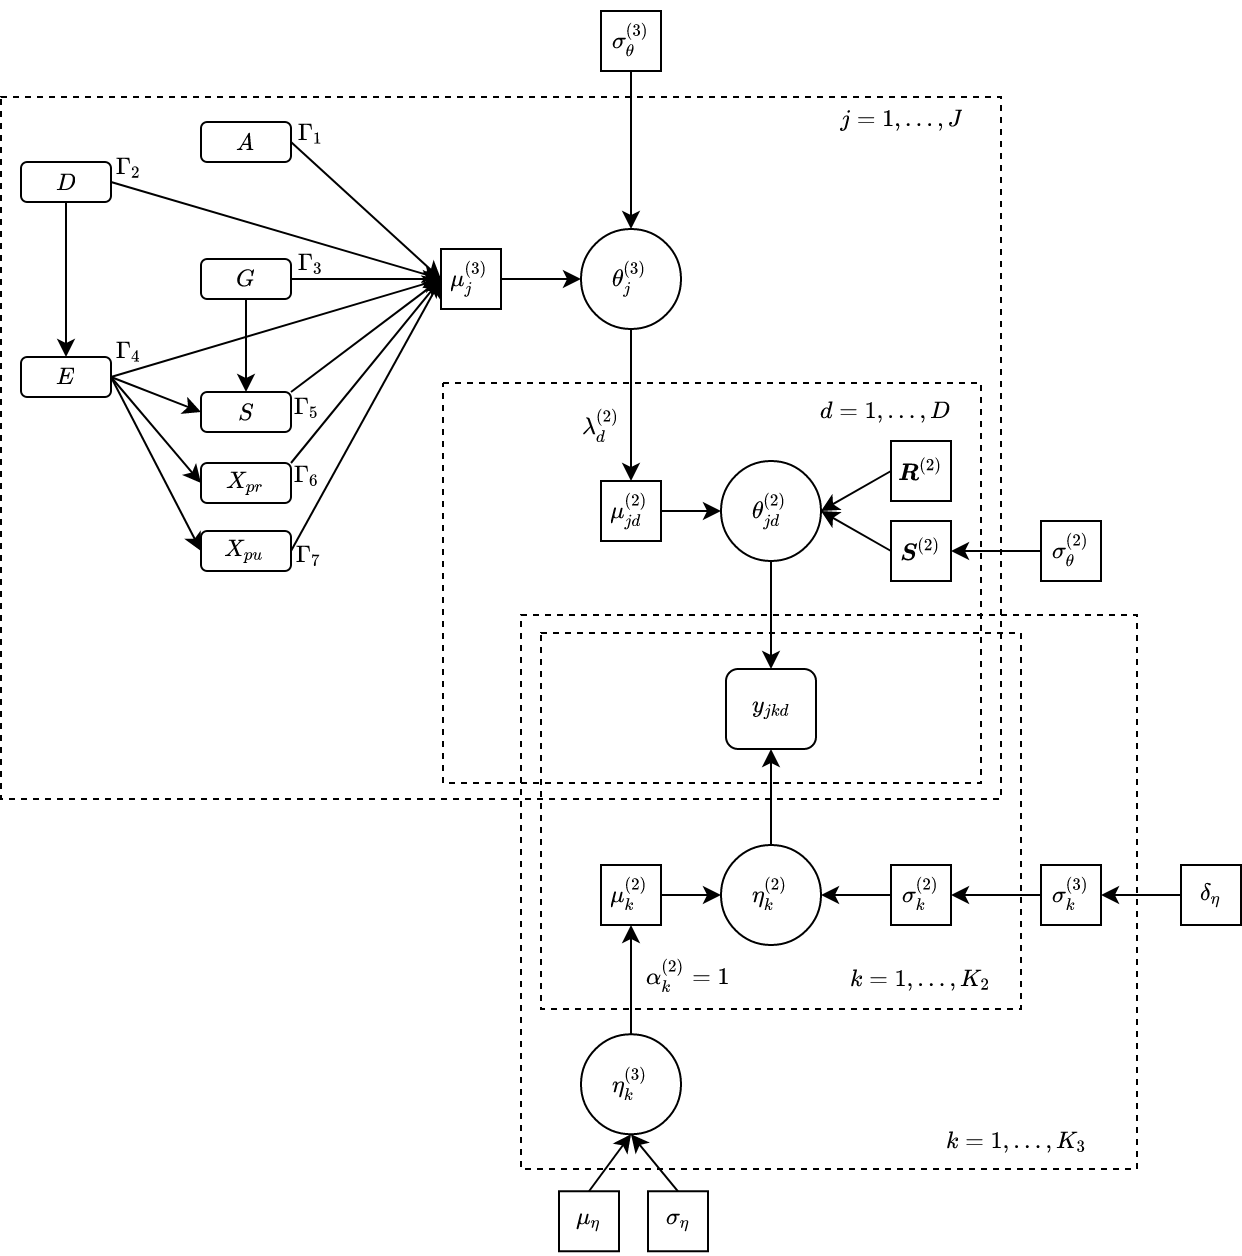
\includegraphics[width=0.8\linewidth]{app_SOLV_dag}
	%
	\caption[Directed Acyclic Graph (DAG). Application's second-order latent variable model (SOLV).]%
	{Directed Acyclig Graph (DAG). Application's second-order latent variable model (SOLV). Circles represent latent variables. Squares represent parameters or parameters for priors. Large squares represent nesting in specific units.}
	\label{fig:SOLV_app}
\end{figure}

Second, we assumed disability ($D$) causally explained the levels of reading comprehension and/or its sub-dimensions. It is not hard to imagine an scenario where this relationship is true, and a good example of this, is people with vision disabilities. As individuals with vision disabilities are forced to learn completely different set of tools and strategies to be able to read and write, e.g. learn Braille or receive text-to-speech support, the possibility that this additional requirements have hindered the individual's development of the reading comprehension abilities is high. Moreover, the possibility that these effect are reflected on their evaluation outcomes is also highly likely. At this point, it is important to indicate that MINEDU provide the means for people with vision disabilities, to be evaluated under equitable conditions, e.g. using evaluation instruments written on Braille or providing text-to-speech support. However, we believe the effects of the disability could offset the effects of the conditions set in place to ensure an equitable evaluation, but we do not know by how much. Furthermore, although the justification to include this variable in the model have been guided by the previous example, one cannot discard that other types of disabilities could also had an impact on the development of the reading comprehension abilities. In this sense, we believe the educational authority only benefits from obtaining this type of evidence, to either target in-training services for these individuals, or to improve further their evaluations conditions, to ensure their participation on the educational workforce. 

Third, we assumed the type of education an applicant received ($E$) affected the reading comprehension abilities, where type of education was a categorical variable that denoted if an individual received his/her pedagogical training from an institute, university, or both. The assumptions behind the inclusion of the variable derives from incidental evidence about the quality of training on pedagogical institutes. In Peru, there is silent, but widely accepted notion that most pedagogical institutes produce teacher with low levels of pedagogical abilities. Multiple reason have been considered, that is, a poorly devised or outdated curricula of teaching; their lack of funding; the fact that mostly institutes are specialized on training people with disabilities; or the fact that because institutes are easier to enter and less expensive than private universities, people coming the lower tiers of income (another proxy of educational opportunities and development), select institutes to begin their education. Considering the previous, it could be of interest for the educational authority to set this incidental evidence on a more quantitative ground, again with the purpose of providing remedial measures. 

At this point, it is important to indicate that from the previous paragraph statements, one can easily assume a backdoor path exists between the education and disability variables (see the path $D \rightarrow E$ on the model's figures). A backdoor path is just a DAG's path that outlines a relationship between two variables, that if remains unchecked can confound the variables' effects on an outcome. In our specific case, this just means that, in order to obtain unbiased estimates for the effects of education and/or disability, both variables need to considered in the model to close any of the backdoor paths.

Fourth, we assumed the educational career experience, measured in years of public or private teaching ($X_{pu}$ and $X_{pr}$, respectively), affected the reading comprehension abilities. In this case, the causal assumption goes in line with the idea that with more teaching experience, the teacher had more opportunities to develop key aspects of the reading comprehension abilities. However, as it happened previously, we believe a backdoor path exist between these covariates and the educational variable. The intuition of these relationships derives from the same incidental evidence relating the type and quality of the pedagogical training. One can imagine, if the pedagogical training in institutes is perceived as of lesser quality, the opportunities a teacher can access, if any, will also be of less quality. We believe the latter is especially true in the private sector, where this perception can also be translated in less years of experience. However, since we are interest in estimating the unbiased and independent effects of education and experience, both set of variables need to be included in the model, as they already are.

Fifth, we assumed the broad definition of teaching specialty ($S$) also explained causally the reading comprehension abilities and/or its sub-dimensions. Specialty was a categorical variable denoting if a teacher had the credentials to instruct at the early childhood, primary, or secondary educational levels. The intuition behind its inclusion, lies in the idea that instructing students that require more complex levels of written and oral communication, could end up benefiting the reading comprehension abilities of teachers. 

Notice from the model's figures, that we have additionally assumed, there is a backdoor path between the specialty and gender variables. In this case, this relationship only tries to reflect that it is more likely that women choose to specialize on the early childhood and primary educational levels. However, it is important to indicate that although gender have been included in the model as a control variable (following a common practice in the literature), our interest is on measuring the total effect of specialty on the abilities. Therefore, to calculate such total effect, we will have to add the direct effect of specialty on the abilities ($\Gamma_{7}$) and the indirect effect of specialty through gender ($\Gamma_{G \rightarrow S} + \Gamma_{6}$).

Therefore, after declaring our hypothesis, we proceed to declare the prior model assumptions related to the aforementioned covariates. We state our current lack of knowledge about the effects of the variables, by setting weakly informative priors, in the following way: 
%
\begin{align}
	\Gamma_{1} &\sim \text{Normal}( 0, 0.5 ) \\
	\Gamma_{2c} &\sim \text{Normal}( 0, 0.5 ) \\
	\Gamma_{3c} &\sim \text{Normal}( 0, 0.5 ) \\
	\Gamma_{4c} &\sim \text{Normal}( 0, 1 ) \\
	\Gamma_{5c} &\sim \text{Normal}( 0, 0.5 ) \\
	\Gamma_{6c} &\sim \text{Normal}( 0, 0.5 )  \\
	\Gamma_{7c} &\sim \text{Normal}( 0, 0.5 ) 
	%
\end{align} 

\noindent where as in the previous chapter, $c$ denotes the categories inside the covariate, different for each variable. 

Finally, by no means we state the proposed model is the ``correct" model to analyze the data. This is particularly true, if we consider that several unobserved important variables are absent from the analysis, e.g. if the individual followed training courses beyond their initial education, or something as simple as, the amount of hours the individual spends on reading. Moreover, this is aggravated by the fact that a good portion of the variables used come from self-reported measures, like experience and education. However, we believe that giving the constraints of the data, the model provides a sensible depiction of the causal hypothesis among the available variables.

%%%%%%%%%%%%%%%%%%%%%%%%%%%%%%%%%%%%%%%%%%%%%%%%%%%%%%%%%%%%%%%%%%%%%%%
%%%%%%%%%%%%%%%%%%%%%%%%%%%%%%%%%%%%%%%%%%%%%%%%%%%%%%%%%%%%%%%%%%%%%%%

\section{Results}

%%%%%%%%%%%%%%%%%%%%%%%%%%%%%%%%%%%%%%%%%%%%%%%%%%%%%%%%%%%%%%%%%%%%%%%

\subsection{Parametrization performance} \label{sub_sect:ergodicity_application}

Figures \ref{fig:FOLV_CE_chains1} and \ref{fig:FOLV_NC_chains1} show the items' trace, trank, and ACF plots for the centered and non-centered parametrization of the application's FOLV model. From a quick inspection of the figures, we realize the items' parameter did not achieved ergodicity under the CP, in contrast to the NCP. This result if further confirmed by figure \ref{fig:FOLV_stat1}, where we observe the items parameters had effective sample sizes below $100$ under the CP, while above $1,500$ under the NCP. Moreover, the parameters' chains registered \texttt{Rhat} values well above the recommended threshold under CP, but maintained values close to one under the NCP.
%
\begin{figure}[H]
	\centering
	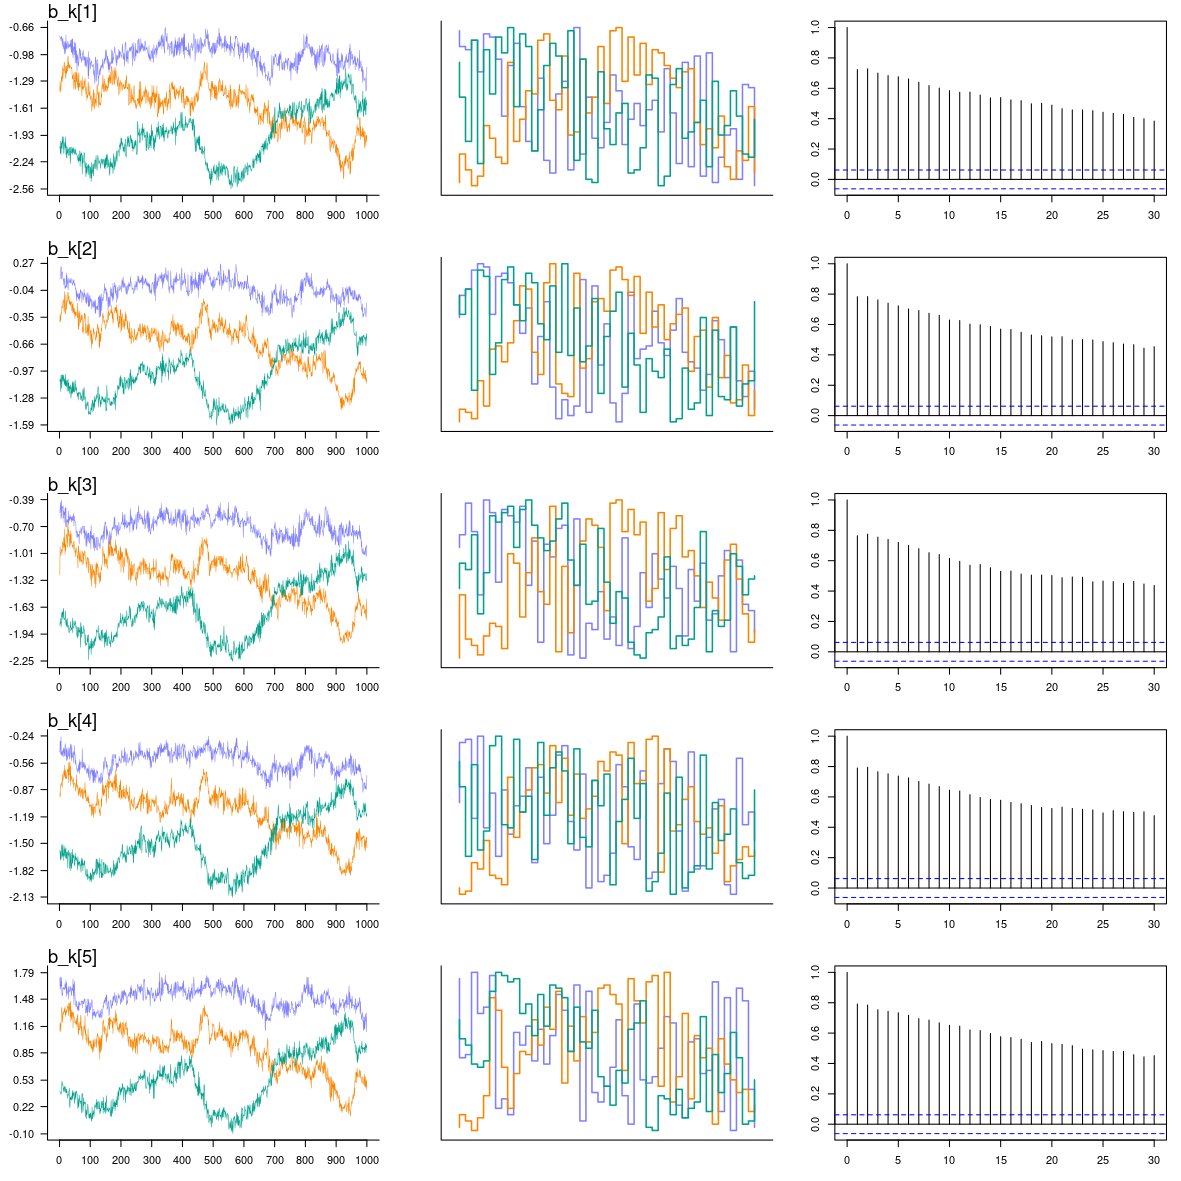
\includegraphics[width=1\linewidth]{FOLV_CE_bk_1_5}
	%
	\caption[Application's first-order latent variable model (FOLV). Centered parametrization. Items difficulty. Trace, trank and auto-correlation plots.]%
	{Application's first-order latent variable model (FOLV). Centered parametrization. Items difficulty: (Left) trace plot, (Middle) trank plot, (Right) auto-correlation plot.}
	\label{fig:FOLV_CE_chains1}
\end{figure}

A similar behavior was registered for the texts difficulties and deviations, and individuals abilities. From the inspection of the appropriate figures\footnote{To inspect the figures refer to the github accompanying page detailed in Appendix \ref{app:chapter5}.}, we notice the CP did not achieved stationarity, convergence, nor good mixing, albeit the patterns were less extreme than in the previous scenario. In contrast, the NCP achieved ergodicity without any issues. Again, this was further confirmed by the comparison of the \texttt{n\_eff} and \texttt{Rhat} values between the two parametrizations.
%
\begin{figure}[H]
	\centering
	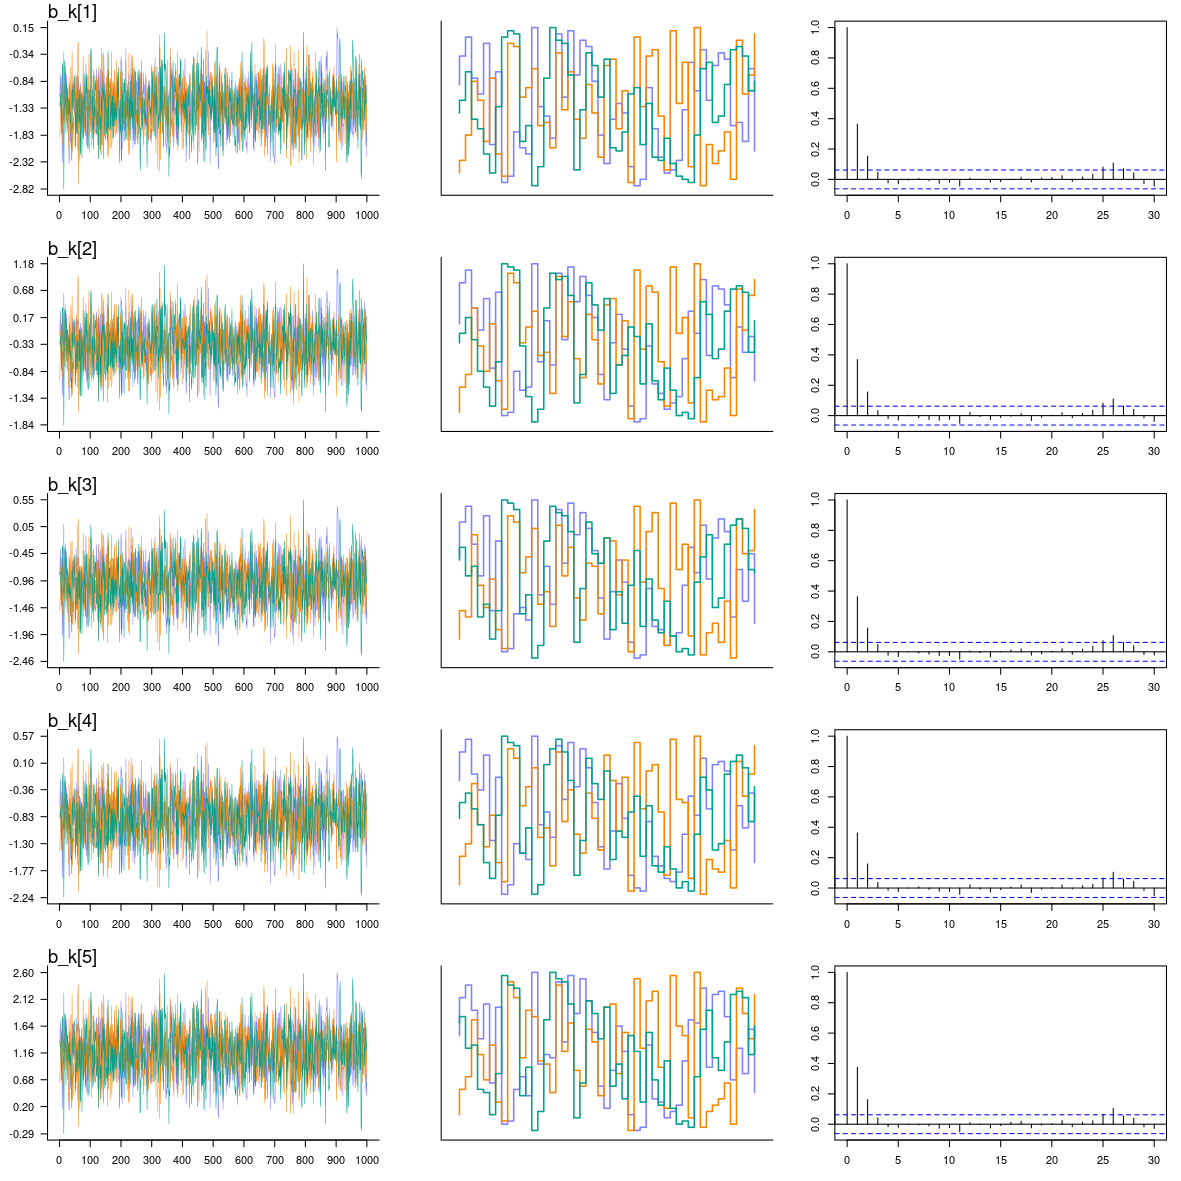
\includegraphics[width=1\linewidth]{FOLV_NC_bk_1_5}
	%
	\caption[Application's first-order latent variable model (FOLV). Non-centered parametrization. Items difficulty. Trace, trank and auto-correlation plots.]%
	{Application's first-Order latent variable model (FOLV). Non-centered parametrization. Items difficulty: (Left) trace plot, (Middle) trank plot, (Right) auto-correlation plot.}
	\label{fig:FOLV_NC_chains1}
\end{figure}

Moreover, both parametrizations had a hard time exploring the posterior distribution of the sub-dimensions correlations. Inspecting the appropriate figures (not shown), we noticed the CP registered effective sample sizes below $100$, while the NCP barely reached sample sizes above $300$. This, in conjunction with the trace, trank, and ACF plots further confirmed the chains did not achieved ergodicity.
%
\begin{figure}[H]
	\centering
	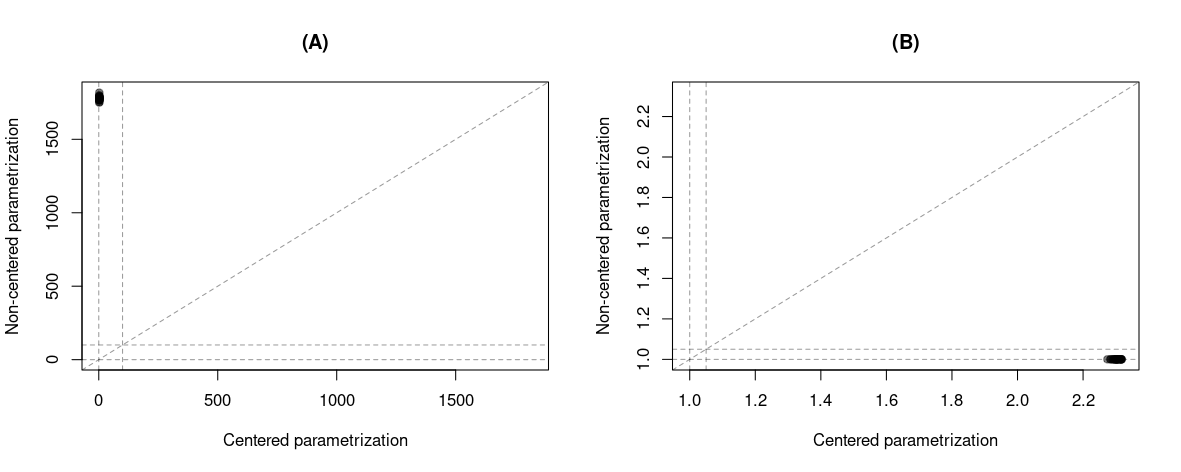
\includegraphics[width=1\linewidth]{FOLV_stat_bk}
	%
	\caption[Application's first-order latent variable model (FOLV). CP and NCP comparison plot.]%
	{Application's first-order latent variable model (FOLV). CP and NCP comparison plot. (A) \texttt{n\_eff} for items' difficulties. (B) \texttt{Rhat} for items' difficulties. Diagonal discontinuous line describes equality between CP and NCP. Vertical and horizontal discontinuous lines set in A corresponds to \texttt{n\_eff}$=100$. Vertical and horizontal discontinuous lines set in B corresponds to \texttt{Rhat}$=1.05$.}
	\label{fig:FOLV_stat1}
\end{figure}

Strikingly similar patterns were observed in the same set of parameters the SOLV shares with the FOLV model. Part of the evidence of such statement can be found in figures \ref{fig:SOLV_CE_appchains1} and \ref{fig:SOLV_NC_appchains1} (appendix). Moreover, the performance patterns of the loadings were similar to the ones observed for the correlations.

All of the preceding results resonate with the performance patterns obtained in the previous chapter. However, in contrast with the results of the simulation study, some of the structural regression parameters (not shown) registered better performance under the CP, rather than the NCP. Among these set of covariates were age, disability, and both of the experience variables. Nevertheless, the disagreement was not unanimous, as the parameters showed ``healthier" chains with larger effective sample sizes, but \texttt{Rhat} values above the recommended threshold, indicating a lack of convergence. This result resonates with \citet{Papaspiliopoulos_et_al_2007}, who stated that the success of the NCP strategy was largely dependent on the specifics of the models and data. Moreover, it is surprising this pattern of behavior was not replicated on the SOLV model, where all of the structural parameters seemed to be more ergodic under the NCP. The latter lead us to think, the previous patterns resulted from the use a possible miss-specified model.

In conclusion, given the results obtained in this section, and section  \ref{sub_sect:ergodicity_simulation} of the previous chapter, conditional on the selected number of iterations, the non-centered parametrization was the only one to ensure the GLLAMM parameters attained ergodicity.

%%%%%%%%%%%%%%%%%%%%%%%%%%%%%%%%%%%%%%%%%%%%%%%%%%%%%%%%%%%%%%%%%%%%%%%

\subsection{Retrodictive accuracy} \label{sub_sect:retrodictive_application}

Much similar to what was the observed in section \ref{sub_sect:retrodictive_simulation} of the simulation study, we notice the model manages to capture the traits of the data, while avoiding its exact replication. Figure \ref{fig:FOLV_pred_app} show the individuals' true proportion of endorsed items, which are within the compatibility intervals of the average and marginal predictions, that is, the observed values for the proportions were close to the predicted mean and outcomes produced by the model. Similarly, we also observe the average and marginal predictions show some level of shrinkage, i.e. the estimates were ``pulled" towards the average true proportion across individuals, in greater or less quantity. As explained in the simulation chapter, this results from the complex pooling of information across individuals, items, texts and dimensions; that allows the model to negotiate between predicting all individuals with the average proportion (under-fitting) or predicting each individual by its own proportion (over-fitting). 
%
\begin{figure}[H]
	\centering
	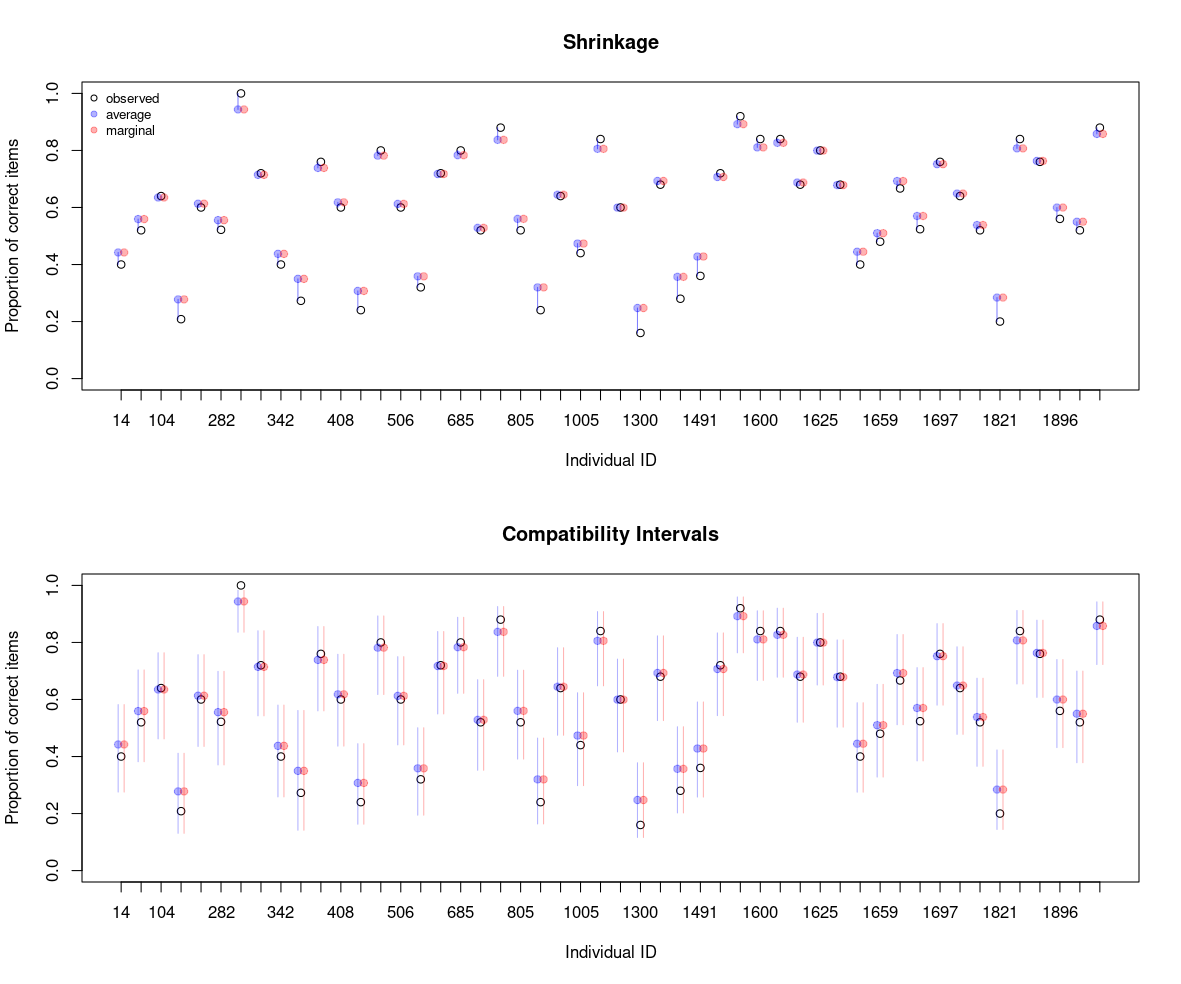
\includegraphics[width=0.9\linewidth]{FOLV_NC_HitRate_ind}
	%
	\caption[First-order latent variable model (FOLV). Non-centered parametrization. Individual predictive plot.]%
	{First-order latent variable model (FOLV). Non-centered parametrization. Individual predictive plot.}
	\label{fig:FOLV_pred_app}
\end{figure}

In a similar fashion, inspecting the appropriate figures (not shown), we can say the retrodictive accuracy of the FOLV model extends to the predicted proportions per individual and covariate combination, as well as proportions aggregated by dimensions, items, and texts\footnote{To inspect the figures refer to the github accompanying page detailed in Appendix \ref{app:chapter5}.}. Furthermore, the SOLV model managed to do a similar job in all of the previous descriptions, as it is evident from figure \ref{fig:FOLV_pred_app}.

Finally, regarding the retrodictive accuracy and model fit, what remains to determine is if the statistical evidence favors one model over the other. This is particularly important, if we notice the SOLV model have approximately $2,000$ more parameters than the FOLV, that is, the reading comprehension abilities of the individuals (not sub-dimensions). In that sense, a lurking fear of over-fitting the data with the SOLV model is present. Additionally, since we implemented our model in a Bayesian framework, the uncertainty of the model fit now has two faces, one resulting from the uncertainty of the parameters, and one coming from to uncertainty of the outcome's likelihood. Therefore, a proper assessment of a model fit would needs to consider these two facets. Lastly, since comparing models based on their training data fit could lead us to wrongful conclusions, we need a method that evaluates our models out-of-sample or through cross-validation, i.e. on data we did not use to train the model's parameters.

Luckily, as \citet{McElreath_2020} indicate, is a benign fact of the statistical theory, that we do not need to re-fit the model multiple times to obtain approximately valid cross-validation measures. Moreover, he continues, is also useful that there are statistics that uses all the information of a ``model's distribution" to asses its fit, and this measures are called information criteria.

It is safe to say that the theory behind the Kullback-Leibler divergence (KL divergence) \cite{Kullback_et_al_1951}, and the field of of information theory in general, from which the information criteria derives, is way out of the scope of the current research. However, the reader can rest assure the information criteria fulfills all the previous requirements to make the proper comparison of our models, more specifically the Pareto-smoothed importance sampling cross-validation (PSIS) \cite{vehtari_et_al_2021} and the Widely Applicable Information Criterion (WAIC) \cite{Watanabe_2013}. Additionally, the reader should keep in mind that as these measures try to approximate the out-of-sample KL divergence, is not the absolute magnitude that matters, but the difference among them. 

Tables \ref{tab:model_fit1} and \ref{tab:model_fit2} show the WAIC and PSIS statistics, respectively. From the tables we notice all models and parametrizations seem to achieve similar levels of out-of-sample prediction, where the penalties again indicate all the models have similar levels of over-fitting risk. Consequently, both models produce similar encodings of the data, therefore, the decision of choosing one over another rest now on a more theoretical ground.
%
\begin{table}[H]
	\centering
	\begin{tabular}{rlrrrr}
		\hline
		& Model & Parametrization & WAIC & lppd & penalty \\  
		\hline\hline
		1 & FOLV & CP &  54,632.4 & -25,429.7 & 1,886.5 \\ 
		2 & FOLV & NCP & 54,631.7 & -25,427.6 & 1,888.3 \\
		%
		\hline
		%
	 	3 & SOLV & CP &  54,610.3 & -25,348.4 & 1,956.7 \\  
		4 & SOLV & NCP & 54,614.7 & -25,337.9 & 1,969.4 \\ 
		\hline
	\end{tabular}
	\caption[Model fit. Widely Applicable Information Criterion (WAIC).]%
	{Model fit. Widely Applicable Information Criterion (WAIC).}
	\label{tab:model_fit1}
\end{table}
%
\begin{table}[H]
	\centering
	\begin{tabular}{rlrrrr}
		\hline
		& Model & Parametrization & PSIS & lppd & penalty \\  
		\hline\hline
		1 & FOLV & CP &  54,657.4 & -27,328.7 & 1,904.4 \\ 
		2 & FOLV & NCP & 54,656.9 & -27,328.5 & 1,898.1  \\
		%
		\hline
		%
		3 & SOLV & CP &  54,627.3 & -27,313.7 & 1,940.1 \\  
		4 & SOLV & NCP & 54,642.5 & -27,321.2 & 1,990.2 \\ 
		\hline
	\end{tabular}
	\caption[Model fit. Pareto-smoothed importance sampling cross-validation (PSIS).]%
	{Model fit. Pareto-smoothed importance sampling cross-validation (PSIS).}
	\label{tab:model_fit2}
\end{table} 


%%%%%%%%%%%%%%%%%%%%%%%%%%%%%%%%%%%%%%%%%%%%%%%%%%%%%%%%%%%%%%%%%%%%%%%

\subsection{Psychometric properties}

As in any standardized evaluation, instrument developers have a special interest in determine how difficult the items were, and in what part of the abilities measurement range they were located. From the top panel of figure \ref{fig:FOLV_CE.NC_recovery}, we notice that the items were scatter throughout a significant portion of the abilities range. However, we also notice the items were more prevalent on the lower tiers, with items located as low as $2.0$ logits.

Finally, an specific benefit of the implementation also allow us to assess how difficult were the texts. The bottom left panel of figure \ref{fig:FOLV_CE.NC_recovery} show the texts difficulties we located around $-0.5$ logits, with large confidence intervals, indicating the items within the texts were scatter in a wide range around the text mean.
%
\begin{figure}[H]
	\centering
	\begin{subfigure}
		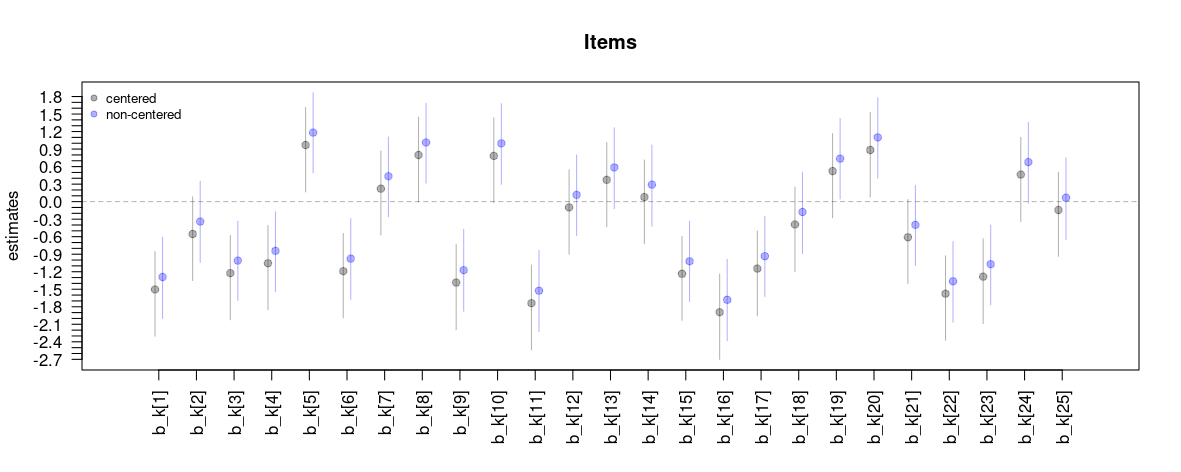
\includegraphics[width=0.9\linewidth]{FOLV_recovery_items}
	\end{subfigure}
	%
	\begin{subfigure}
		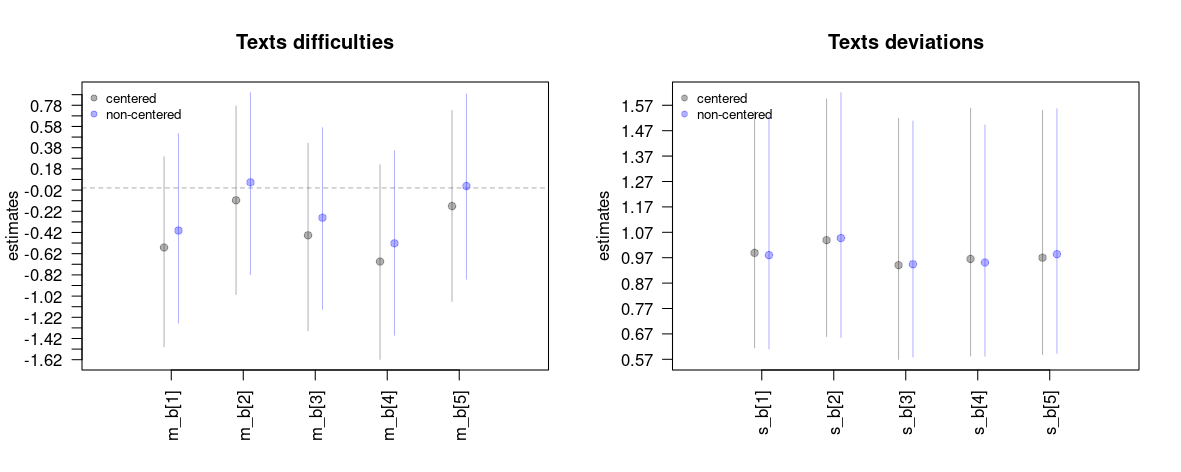
\includegraphics[width=0.87\linewidth]{FOLV_recovery_texts}
	\end{subfigure}
	%
	\caption[Application's first-order latent variable model (FOLV). Centered and non-centered parametrization. Items, and texts difficulties, and texts deviations.]%
	{Application's first-order latent variable model (FOLV). Centered and non-centered parametrization. Items, texts difficulties, and texts deviations.}
	\label{fig:FOLV_CE.NC_recovery}
\end{figure}


%%%%%%%%%%%%%%%%%%%%%%%%%%%%%%%%%%%%%%%%%%%%%%%%%%%%%%%%%%%%%%%%%%%%%%%

\subsection{Test hypothesis} \label{sect:test_hypothesis}

Finally, we investigate the hypothesis 

explain age, not included
%
\begin{figure}[H]
	\centering
	\begin{subfigure}
		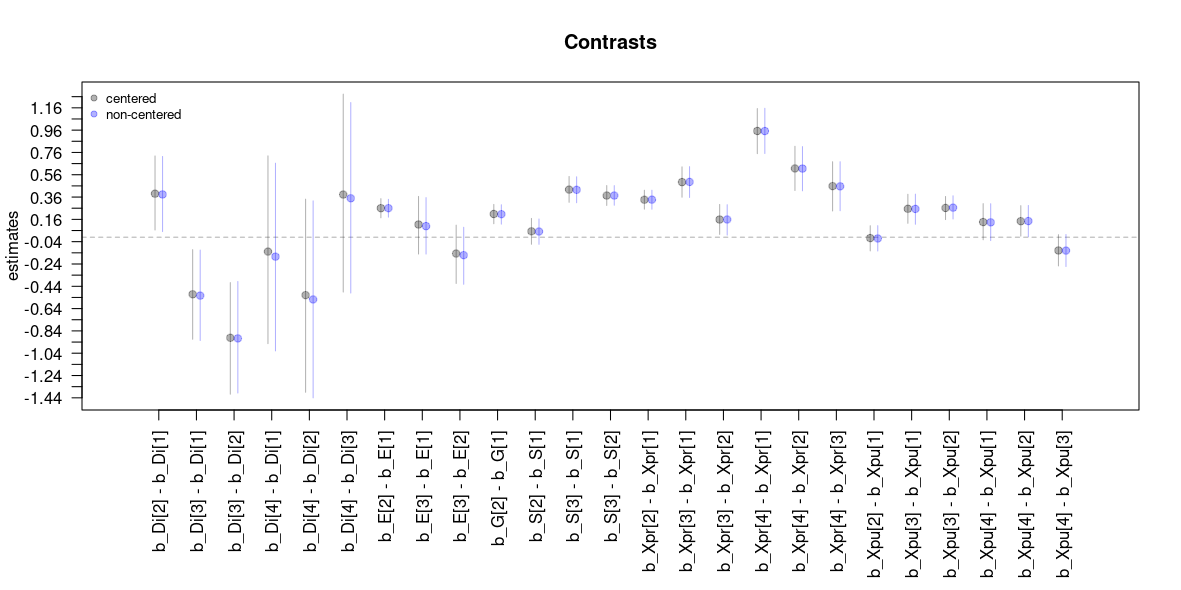
\includegraphics[width=0.9\linewidth]{FOLV_recovery_contrast}
	\end{subfigure}
	%
	\begin{subfigure}
		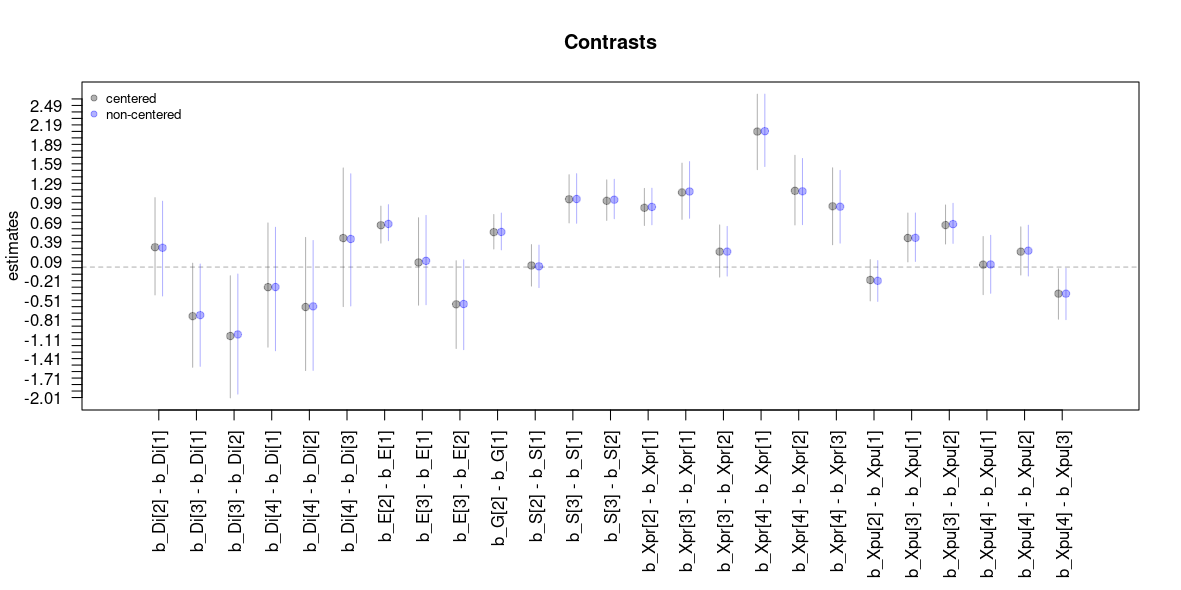
\includegraphics[width=0.9\linewidth]{SOLV_recovery_contrast}
	\end{subfigure}
%
	\caption[Application's first- and second-order latent variable model. CP and NCP comparison plot.]%
	{Application's first- and second-order latent variable model. CP and NCP comparison plot. (Top panel) Contrasts in the FOLV model. (Bottom panel) Contrasts in the SOLV model. }
	\label{fig:contrast_both}
\end{figure}






